%%%%%%%%%%%%%%%%%%% 使用Latexmk编译 %%%%%%%%%%%%%%%%%%%%%%%

\documentclass[10pt]{article}
\usepackage{ctex}
\usepackage{NotesTeXV3,lipsum}
\usepackage{graphicx}
%\usepackage{showframe}
\begin{document}
    \title{通信电子线路}
	\author{}
	\maketitle
	\newpage
%    \pagestyle{fancynotes}
    \part{绪论}
    \section{非线性电子线路的作用}
    利用器件的非线性完成振荡、频率变换等功能的电路统称为非线性电子线路。
    非线性电子线路分为3类:功率放大器、振荡器、调制解调器

    \par
   电磁波的传播方式:
   \begin{enumerate}
    \item 沿地表 \quad $1.5MHZ$ \quad $\lambda > 200m$
    \item 电离层反射 \quad $1.5MHZ ~ 30MHZ$ \quad $10 m <\lambda < 200m$\quad (传播距离、时间最长)
    \item 沿直线传播波 \quad $30MHZ$以上 \quad $\lambda < 10m $
   \end{enumerate} 

   \par
   无线通信系统由发射装置、接收装置和传输媒质组成。\\
   发射装置包括:换能器、发射机、发射天线。
   \begin{figure}[H] %H为当前位置,!htb为忽略美学标准,htbp为浮动图形
    \centering %图片居中
    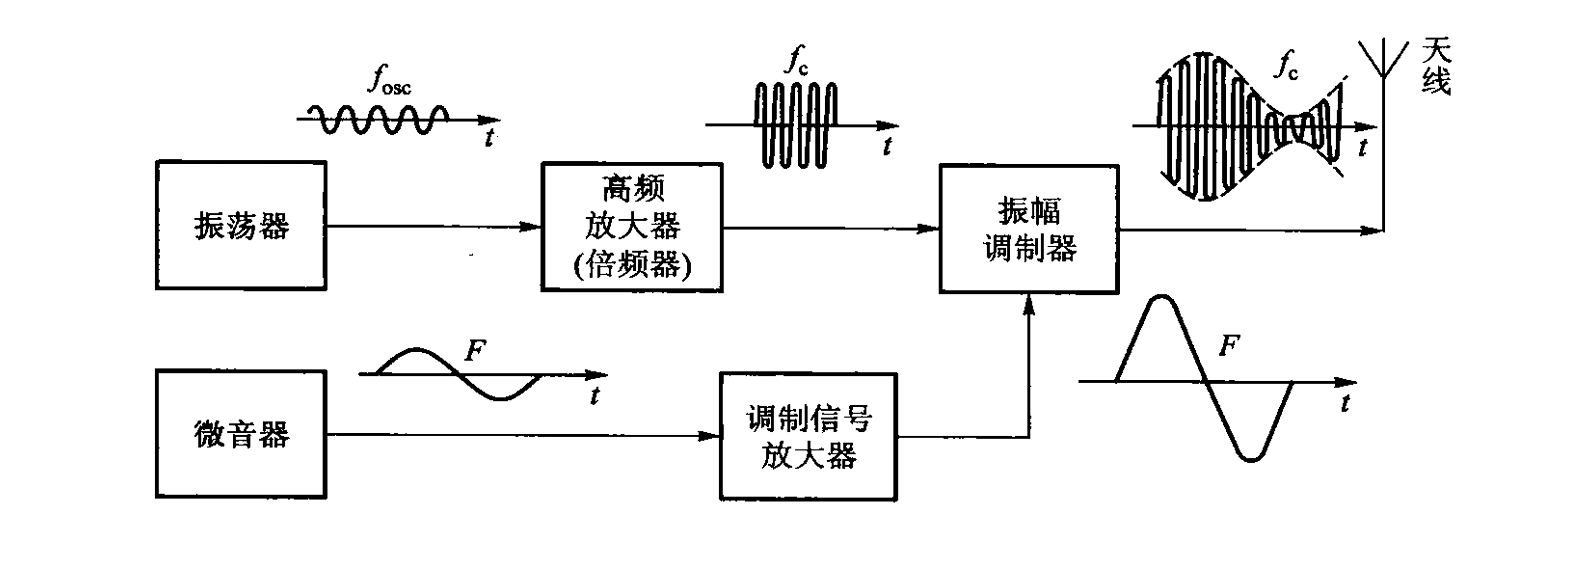
\includegraphics[width=0.7\textwidth]{pictures/1-1.png} %插入图片,[]中设置图片大小,{}中是图片文件名
    \caption{采用调幅方式的发射机组成框图} %最终文档中希望显示的图片标题
    \label{fig.1-1} %用于文内引用的标签
    \end{figure}
    \marginnote{调制型号放大器(又称低频放大器),由多级放大器组成,前面几级为小信号放大器,后面几级为功率放大器}
   接收装置包括:接收天线、接收机、换能器
   \begin{figure}[H] %H为当前位置,!htb为忽略美学标准,htbp为浮动图形
    \centering %图片居中              
    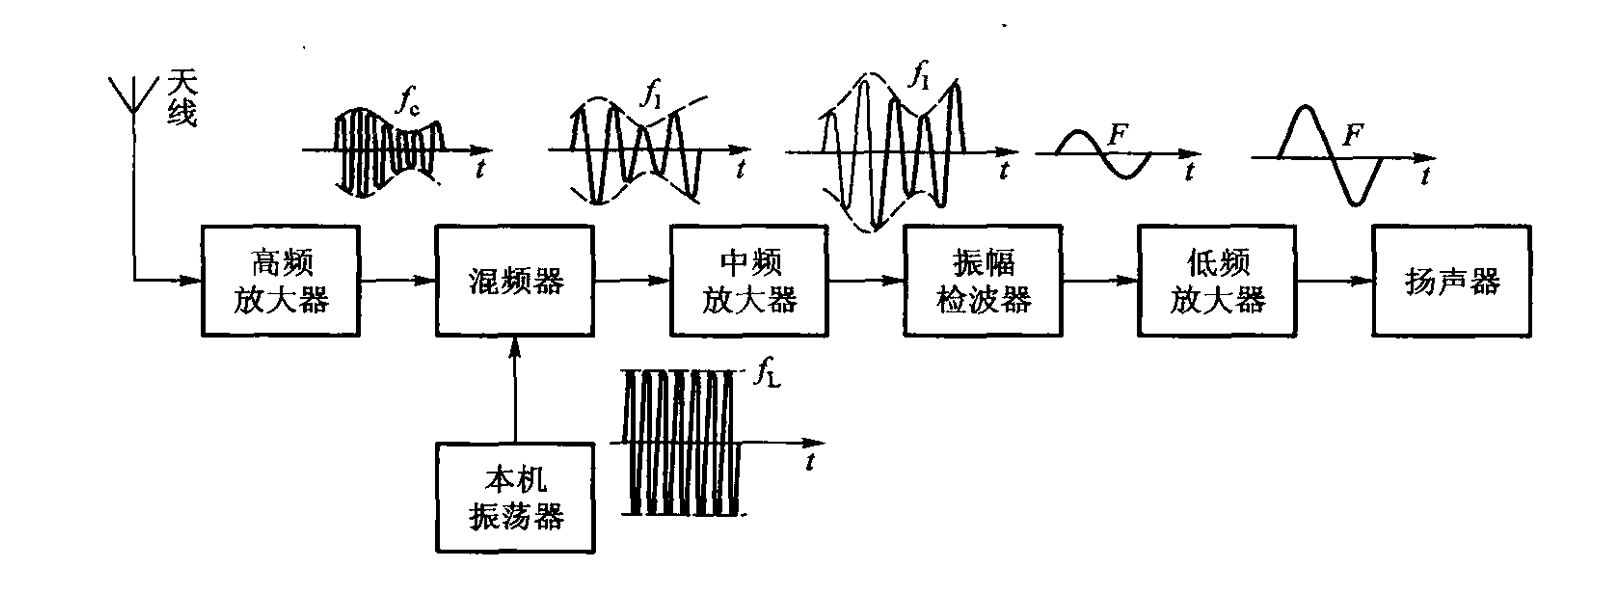
\includegraphics[width=0.7\textwidth]{pictures/1-2.png} %插入图片,[]中设置图片大小,{}中是图片文件名
    \caption{采用调幅方式的接收机组成框图(超外差式)} %最终文档中希望显示的图片标题
    \label{fig.1-1} %用于文内引用的标签
    \end{figure}
    \marginnote{混频器可以提高解调能力,$f_I = |f_L - f_c|$ 为一固定数值}
    调制有调辐、调频、调相三种,调频和调相统称为调角。携带有信息的电信号称为调制信号,未调制的高频振荡信号称为载波信号。
    经过调制后的高频振荡信号称为已调波信号。\par
    解调是调制的逆过程,将已调波信号变换为携带信息的电信号。\par
    只有信号波长与天线尺寸可以比拟的时候,天线才能有效辐射和接收电磁波,调制可以显著减小天线尺寸。
    调制可以电信号载到不同频率的载波信号上,接收机就可以根据频率选出信息,抑制其他信息干扰。
\section{非线性器件的基本特点}
    直流电导:\par
    $$
    g_0 |_Q = \frac{I_Q}{V_Q}
    $$
    交流电导/增量电导/微变电导:\par
    $$
    g|_Q = \frac{di}{dv}
    $$
    平均电导:基波电流振幅与外加电压振幅的比值
    $$
    g_{av}|_{Q,V_m} = \frac{I_{1m}}{V_m}
    $$

   \begin{figure}[H] %H为当前位置,!htb为忽略美学标准,htbp为浮动图形
    \centering %图片居中
    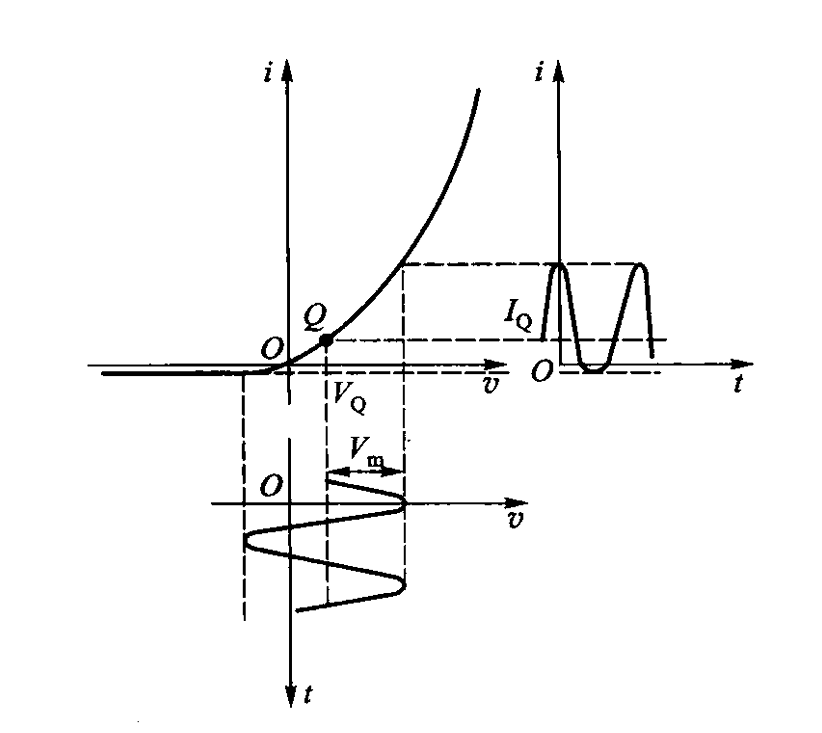
\includegraphics[width=0.7\textwidth]{pictures/1-3.png} %插入图片,[]中设置图片大小,{}中是图片文件名
    \caption{$g_{av}$定义} %最终文档中希望显示的图片标题
    \end{figure}

 非线性器件不满足叠加定理

\newpage
\part{功率电子线路}
\section{功率电子线路概述}
\subsection{功率放大器}
功率放大器的要求:安全、高效、不失真地输出所需信号功率\par
功率放大器是能量转化器,直流电源提供直流功率$P_D$,一部分转化为输出信号功率$P_o$,其余部分小号在集电极。
集电极效率$\eta_C$,定义为:
$$
\eta_C = \frac{P_o}{P_D} = \frac{P_o}{P_o + P_C}
$$

功率管的应用状态:
\begin{table}[h]
    \centering
    \begin{tabular}{|c|c|c|c|c|}
    \hline
    类型 & 甲类 & 乙类 & 甲乙类&丙类 \\
    \hline
    导通时间 & 一个周期 & 半个周期 &甲类和乙类之间& 小于半个周期 \\
    \hline
    \end{tabular}
    \caption{各种状态下的导通时间}
    \label{tab:example}
\end{table}

\begin{figure}[H] %H为当前位置,!htb为忽略美学标准,htbp为浮动图形
 \centering %图片居中
 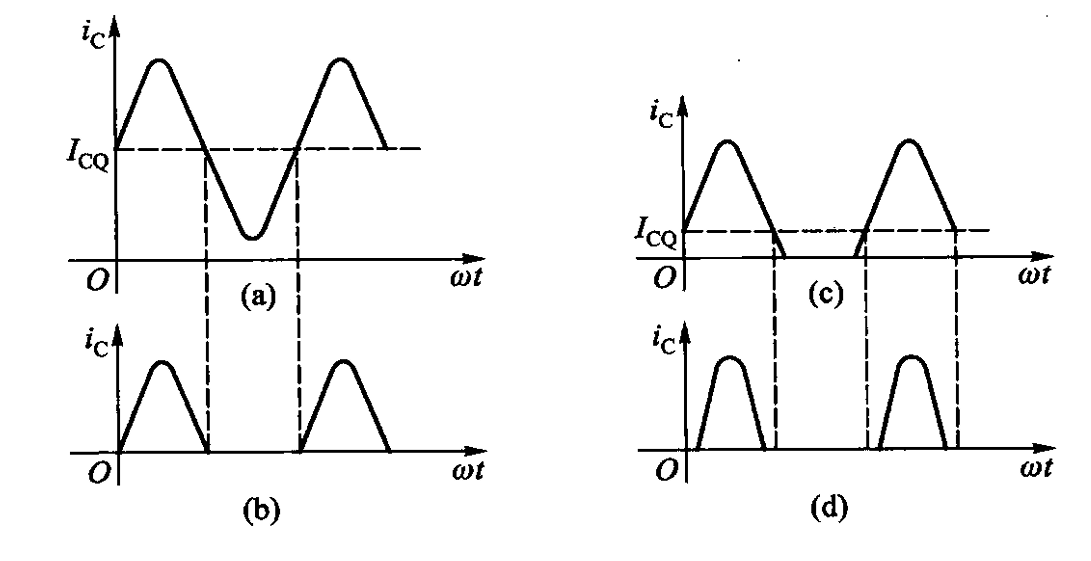
\includegraphics[width=0.7\textwidth]{pictures/2-1.png} %插入图片,[]中设置图片大小,{}中是图片文件名
 \caption{(a)甲类\quad(b)乙类\quad(c)甲乙类\quad(d)丙类 } %最终文档中希望显示的图片标题
 \label{fig.1-1} %用于文内引用的标签
 \end{figure}

 集电极耗散功率$P_C$:
 \begin{equation}
   P_C = \frac{1}{2\pi} \int_{0}^{2\pi} i_Cv_{CE} \, dt
\end{equation}
减小管子在一个周期内的导通时间可增大效率,$\eta_C$丙类$>$乙类$>$甲类,该效率的运用状态都是波形严重失真。、
\par
\subsection{电源变换电路}
\normalsize
\begin{enumerate}
    \item 整流器:交流变直流
    \item 直流-直流变换器
    \item 逆变器:直流变交流
    \item 交流-交流变换器
\end{enumerate}
\subsection{功率器件}
功率器件:散热、$P_{CM}$、二次击穿要看一下
\section{功率放大器的电路组成和工作特性}
功率管为大信号工作,性能分析时必须用大信号模型。工程上多用图解分析法。
\begin{example}
    以基本放大器为例,分析功率性能。
\begin{figure}[H] %H为当前位置,!htb为忽略美学标准,htbp为浮动图形
 \centering %图片居中
 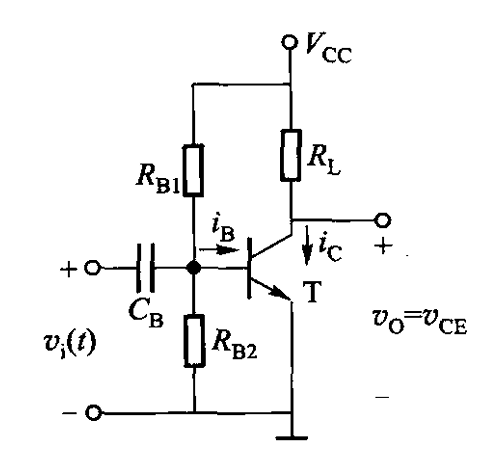
\includegraphics[width=0.4\textwidth]{pictures/2-2.png} %插入图片,[]中设置图片大小,{}中是图片文件名
 \caption{基本放大器} %最终文档中希望显示的图片标题
 \label{fig.2-2} %用于文内引用的标签
 \end{figure}
假设忽略$V_{CE(on)}$和$I_{CEO}$,
设工作点$V_{CEQ} = \frac{V_{CC}}{2}$,$I_{CQ} = \frac{V_{CEQ}}{R_L} = \frac{V_{CC}}{2R_L}$ 
在最大幅值的情况下($v_{im} = \frac{V_{CC}}{2}$)
\begin{align*}
    i_C &= I_{CQ} + I_{cm}\sin(\omega t) \\
    v_{CE} &= V_{CEQ} - v_{cm}\sin(\omega t)
\end{align*}
直流功率$P_D$,负载功率$P_o$,集电极功率$P_C$,分别为
\begin{align}
P_D = \frac{1}{2\pi}\int_{0}^{2\pi}V_{CC}i_{C}dt = V_{CC}I_{CQ}\\
P_L = \frac{1}{2\pi}\int_{0}^{2\pi}i_{C}^2R_L d\omega t  = V_{CEQ}I_{CQ}+\frac{1}{2}V_{cm}I_{cm}\\
P_C =  \frac{1}{2\pi}\int_{0}^{2\pi} v_{CE}i_{C} = V_{CEQ}I_{C}-\frac{1}{2}V_{cm}I_{cm}
\end{align}
\end{example}

\marginnote{$P_o$是负载的得到的信号功率,$P_L$是负载得到的所有功率,有交流和直流两部分,
只有交流部分(信号功率$P_o$)是希望得到的}
$P_D$只于电源电压和工作点有关,$P_L$ 和 $P_C$都由交流和直流两部分组成,且表达式相同,只是$P_L$是加交流功率,$P_C$是减。
$P_L$的交流项为$P_o = \frac{P_D}{4}$,只有这一部分是希望输出的。如果不加信号,管子的负载功率和集电极功率相同,加上信号后,
集电极减少的功率即为负载所得的信号功率。\par
基本放大器的集电极最大功率
$$
\eta_{Cmax} = \frac{P_o}{P_D} = \frac{1}{4} = 25\%
$$
如果考虑$V_{CE(sat)}$和$I_{CEO}$,该效率会更低,另外,功率管的集电极饱和压降$V_{CE(sat)}$会大于$0.3V$
上面分析表明:电源的功率一部分消耗在管子中,大部分($\frac{P_D}{2}$)作为直流功率消耗在$R_L$,
可以采用以下方法减少消耗:
\begin{enumerate}
    \item 改变功率管的运用状态(甲乙类、乙类)。(减少功率管本身消耗的功率)
    \item 管外电路采用不消耗直流功率的结构。(减少直流功率消耗)
\end{enumerate}
同时,$v_{CE}$最大振幅一定,可以减小$R_L$使负载线变陡,提高工作点电流,在这时提高输入激励$i_b$振幅,
使输出$i_C$增大。
\begin{figure}[H] %H为当前位置,!htb为忽略美学标准,htbp为浮动图形                                   begin{figure}
  \centering %图片居中
  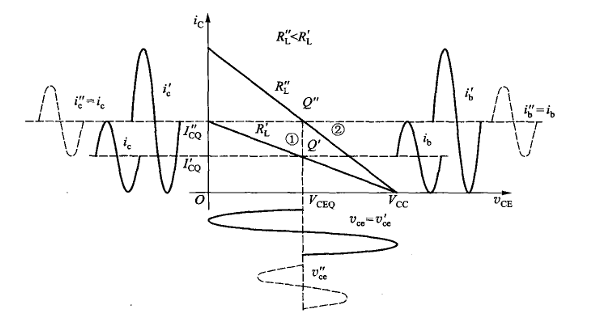
\includegraphics[width=0.4\textwidth]{pictures/2-5.png} %插入图片,[]中设置图片大小,{}中是图片文件名
  \caption{$R_L$改变对$i_C$的影响} %最终文档中希望显示的图片标题
  \label{fig.2-5} %用于文内引用的标签
\end{figure}
\par
在不改变功率管运用状态的条件下,管外使用不消耗直流功率的结构,就是甲类功率放大器。
\subsection{甲类功率放大器}
\subsection{乙类功率放大器}
根据甲类功放的分析结论可知,降低工作点可以提高效率。将管子的工作点设置在0,就得到了乙类功放。
乙类功放没有直流损耗,只有在有信号时才有损耗。
不过,功率管只有在导通时才有电流流过,因为工作点为0,所以只有在输入激励在正半周期时,功率管导通,才
有电流流过,所以输出只有半个周期,是失真的。
为了得到完整的正弦波,高频时可以利用谐振回路选出其基波,低频时采用两只管子轮流导通的推挽电路,
两个半波在负载上合成一个完整的正弦波。下面是两种典型电路。
    \begin{enumerate}
        \item 变压器耦合
        \item 互补推挽
    \end{enumerate}
\begin{example}
    \begin{enumerate}
    \item 变压器耦合:图(a)
    输入变压器$Tr_1$利用中心抽头接地,将输入电压分为两个大小相等、对地极性相反的激励信号
    实现$T_1$管和$T_2$管轮流导通:输入信号正半周期时,$v_{i1}>0$,$v_{i2}<0$,$T_1$管导通,
    $T_2$管截止,输入信号为负半周期时,正好相反。
    因为$i_{C1}$和$i_{C2}$方向相反,所以两个电流的直流部分相互抵消。
    交流部分通过变压器在负载上合成为一个完整正弦波\par
    \begin{figure}[H]
        \centering
        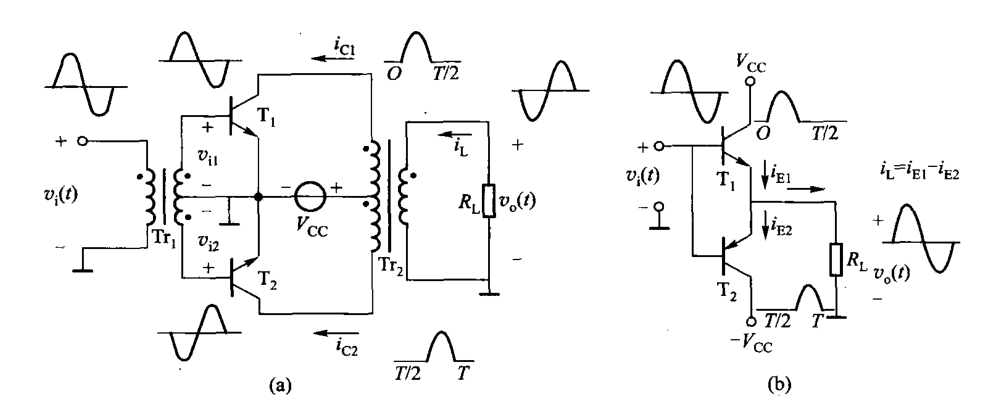
\includegraphics[width=0.7\textwidth]{pictures/2-7.png}
        \caption{两种乙类推挽功放}
    \end{figure}
    \item 互补推挽:图(b)\par
    互补推挽电路使用了连个特性配对的互补功率管,使用等值正负电源($+V_{CC},-V_{CC}$)供电。
    无信号时两管|$V_{CE}$|相同,所以$V_{CE1} = +V_{CC}, V_{CE2} = -V_{CC}$,且$O$点电位为$0$。
    输入信号正半周期时,$T_1$管导通,$T_2$管截止,$i_{E1}$为向右的正半周期$i_{e1}$和直流部分
    输入信号负半周期时,$T_1$管截止,$T_2$管导通,$i_{E2}$为向左的正半周期$i_{e2}$和直流部分
    \marginnote{向左的正半周期相当于向右的负半周期}
    $i_{E1}$和$i_{E2}$直流部分相互抵消,交流部分在负载上合成为一个完整正弦波。
    \end{enumerate}
\end{example}

\par
因为两管时特性配对(对称)的,所以只需要对其中一个分析即可。
考虑直流通路时,输入信号接地,两管基极直流电压都为$0$,$V_{BE} = 0$,$I_C = 0$,两管都工作在
乙类状态,静态工作点分别在$+V_{CC}$和$-V_{CC}$上。
$T_{1}$管导通时交流负载线是一条斜率为$\frac{1}{R_L}$的直线。


\[
\text{最大集电极效率} \eta_C
\left\{
\begin{array}{lll}
\text{基本放大器:} & 25\% & \\
\text{甲类功放:} & 50\% & \\
\text{乙类功放:} & 78.5\% \ (\frac{\pi}{4}) & \\
\end{array}
\right.
\]
\section{整流电路}
\begin{figure}[H]
    \centering
    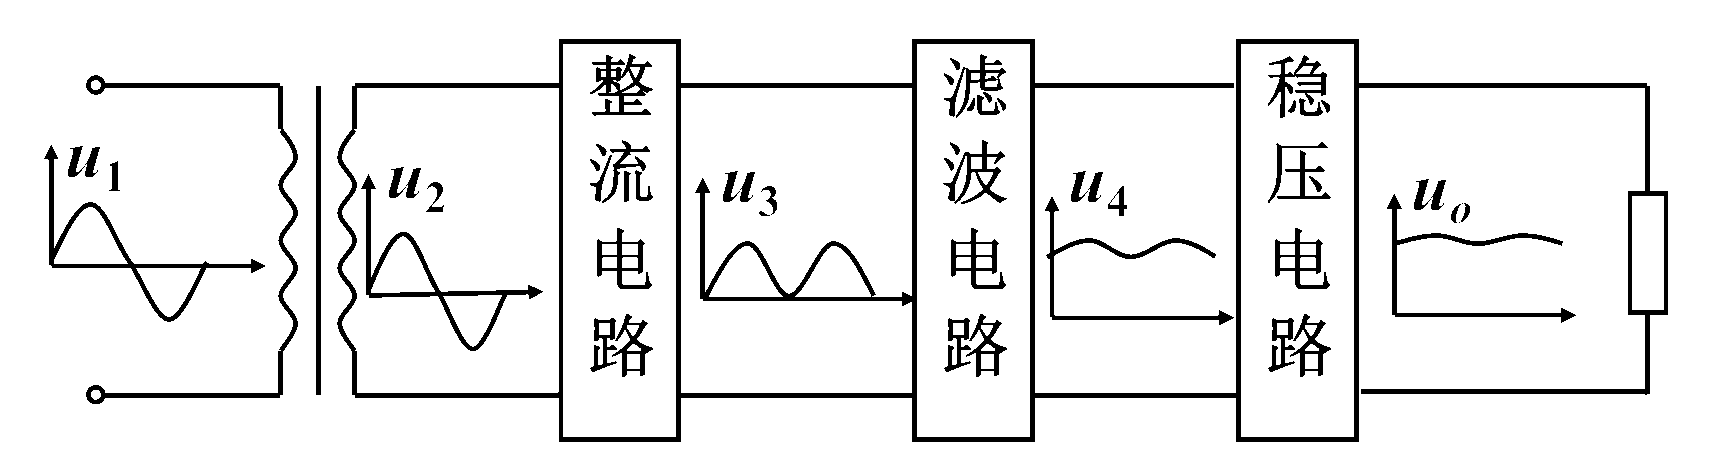
\includegraphics[width=0.7\textwidth]{pictures/bw-2-6.png}
    \caption{直流稳压电源的组成}
\end{figure}


\section{稳压电路}
\subsection{串联稳压电路}
串联稳压电路是由调整管、取样管、基准电压源、比较放大器组成的自动控制电路。
\subsection{开关稳压电路}

\newpage
\part{谐振功率放大器}
\section{谐振功率放大器工作原理}
\section{实际电路设计}
\subsection{直流馈电电路}
原则:保证直流电流只流过直流电源、保证交流电流不流过直流电源\par
直流馈电电路有两种不同的链接方式,分别称为串馈和并馈。
串馈:$V_{CC}$、谐振回路、三极管再同一条回路上。
并馈:$V_{CC}$、谐振回路、三极管不能组成一条回路。
两种馈电方式具有相同的直流通路。串馈电路中,滤波匹配网络处于直流高电位,网络器件不能直接接地,
并馈电路中,由于$C_{C1}$隔直流的作用,滤波网络处于直流低电位,网络器件可以直接接地,所以安装比
串馈方便,但$L_{C}$和$C_{C1}$的分布参数将直接影响网络谐振
\begin{example}
    集电极馈电线路:
 \begin{figure}[H] %H为当前位置,!htb为忽略美学标准,htbp为浮动图形
  \centering %图片居中
  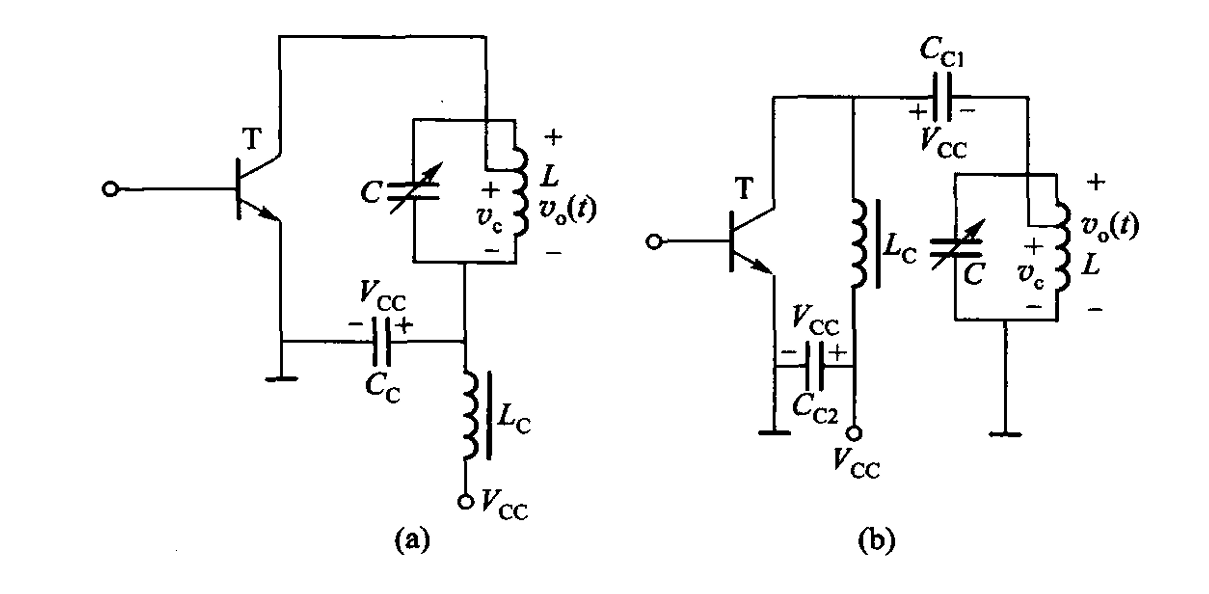
\includegraphics[width=0.4\textwidth]{pictures/2-3.png} %插入图片,[]中设置图片大小,{}中是图片文件名
  \caption{集电极馈电线路} %最终文档中希望显示的图片标题
  \label{fig.2-3}%用于文内引用的标签
 \end{figure}
 (a)交流分量从电容处流走,但是仍会有少部分交流分量流经电源,加入高频扼流圈组阻止交流通过。
 (b)
\end{example}
$V_{CC}$和$V_{BB}$的共同作用是偏置,$V_{CC}$多一个作用是提供功率,如果$V_{BB}$
是从$V_{CC}$上引入的话就可以少用一个电源。\par
将$V_{BB}$删去,$V_{BB}$由电路本身获得

$$
\left\{  
    \begin{array}{cc}  
        V_{BB} < 0 & \text{丙类}\\  
        V_{BB} = 0\\  
        V_{BB} > 0\\    
    \end{array}  
\right.  
$$

\begin{example}
基极偏置电路
\begin{figure}[H] %H为当前位置,!htb为忽略美学标准,htbp为浮动图形
    \centering %图片居中
    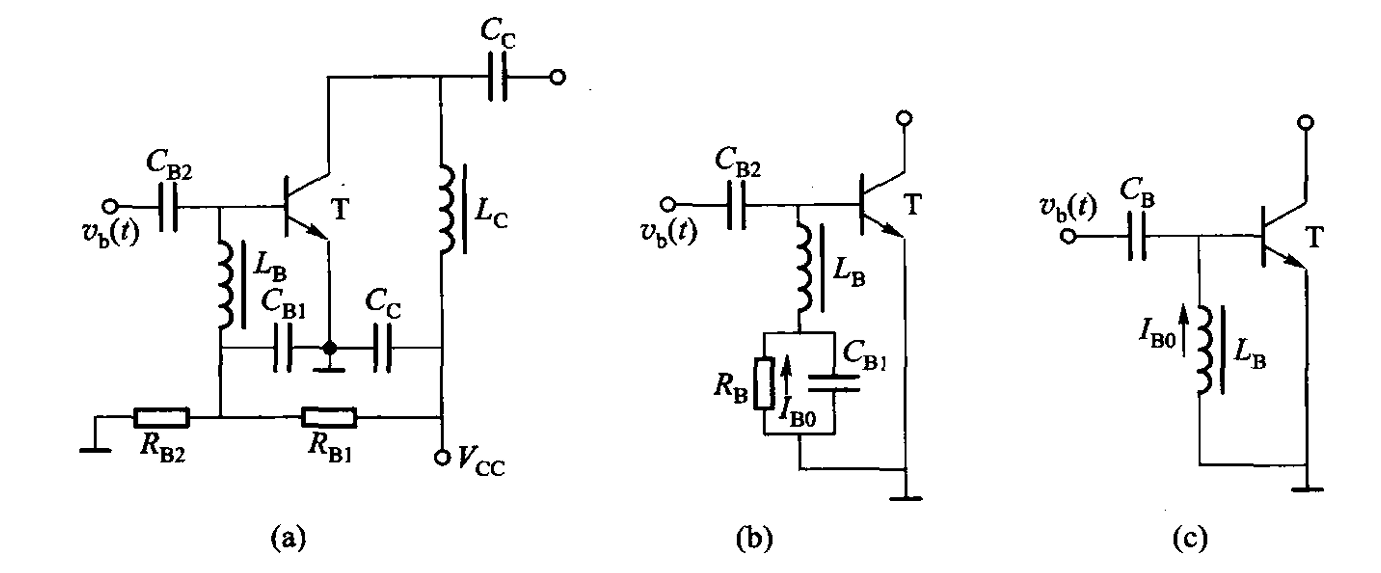
\includegraphics[width=0.7\textwidth]{pictures/2-4.png} %插入图片,[]中设置图片大小,{}中是图片文件名
    \caption{集电极馈电线路} %最终文档中希望显示的图片标题
    \label{fig.2-4}%用于文内引用的标签
\end{figure}
\begin{enumerate}
\item (a):正偏置,偏置$V_{CC}$经过两个电阻分压之后得到,图中$V_{BB}$是$R_{B2}$的分压
$V_{BB}$永远大于0。为保证丙类工作,其值应小于功率管的导通电压。
\item (b):负偏压,不引入$V_{CC}$,由电路自己产生偏置。$I_{B}$从三极管基极进入,
$I_{B}$可分为直流分量、一次谐波分量、二次谐波分量$\dots$,电阻通直流$I_{B0}$,
产生的压降作为$V_{BB}$,$V_{BB}$。
\item (C):零偏压,没有电阻,残生不了压降,$V_{BB}  = 0$
\end{enumerate}
\end{example}
(a)是固定偏压,(b)和(c)是自给偏压。
负偏压的$V_{BB}$很小,因为$I_{B0}很小$
改进:电阻并电容的回路搬到发射极,因为$i_e = \beta i_b$,
电流增大了一百($\beta$)倍,但是不接地了,$V_{BB}$依然$<0$
$$
\text{基极偏置电路}
\left\{  
    \begin{array}{cc}  
        \text{分压偏置}\\  
        \text{自给偏置} \left\{
            \begin{array}{cc}
                \text{负偏压}\\
                \text{零偏压}
            \end{array}
        \right.
    \end{array}  
\right.  
$$

\subsection{滤波匹配网络}
滤波匹配网络使功率$P_o$最有效的输出。在电路中学过,如果一个电压源外接一个电阻,
当外接电阻与内阻相同时,电压源输出功率最大。滤波匹配网络的目的就是使网络谐振时的电阻等于负载电阻。
滤波匹配网络分为并脸型和串联型。
\par 先看并联谐振网络


$$
\text{并联谐振网络}
\left\{  
    \begin{array}{cc}  
        \text{变压器}\\  
        \text{LC网络}
    \end{array}  
\right.  
$$
  \begin{enumerate}
   \item 变压器:通过调节抽头
  \end{enumerate} 



\end{document}
